\chapter{Metodologi Penelitian}

Berdasarkan rumusan masalah, ruang lingkup penelitian, serta batasan penelitian yang sudah dibahas pada bab sebelumnya, berikut ini adalah metodologi penelitian yang penulis gunakan:

\begin{figure}
    \centering
    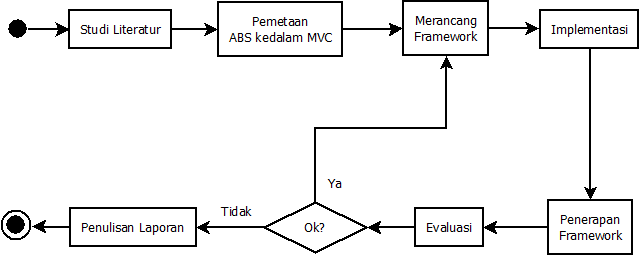
\includegraphics[width=0.8\textwidth]
        {img/metodologi-penelitian.png}
    \caption{Rencana Penelitian}
    \label{fig:metodologiPenelitian}
\end{figure}

Seperti yang terlihat pada Gambar \ref{fig:metodologiPenelitian} diatas, pada awal penelitian penulis melakukan studi literatur untuk mendapatkan pengetahuan terkait teori-teori pendukung yang penulis gunakan dalam melakukan penelitian. Setelah selesai melakukan studi literatur, berikutnya penulis melakukan proses analisa dan pemetaan terhadap bahasa pemodelan ABS untuk kemudian dilakukan pemetaan kedalam komponen-komponen MVC. Seteah proses pemetaan selesai, penulis membuat rancangan ABS MVC Framework sesuai dengan hasil analisa dan pemetaan yang telah dilakukan dan setelah itu penulis melakukan proses implementasi untuk merealisasikan desain yang telah dibuat. Langkah berikutnya adalah melakukan proses penerapan ABS MVC Framework untuk melihat apakah \textit{framework} yang dibuat dapat digunakan untuk membuat sebuah aplikasi berbasis web dan melakukan evaluasi terhadap \textit{framework} tersebut untuk menentukan apakah harus dilakukan perombakan atau sudah layak sebagai sebuah MVC Framework. Berikut ini adalah detail dari setiap tahapan penelitian yang penulis lakukan:

\section{Studi Literatur}

Pada tahap ini penulis melakukan studi literatur dari berbagai sumber seperti buku, artikel ilmian dan web untuk mendapatkan informasi dan pengetahuan terkait teori pendukung yang penulis butuhkan dalam melakukan penelitian ini. Adapun pengetahuan-pengetahuan pendukung yang penulis butuhkan antara lain adalah pengetahuan tentang Hypertext Transfer Protocol (HTTP), pola Model-View-Controller (MVC) dalam pengembangan perangkat lunak, pengetahuan tentang bahasa pemodelan ABS dan pengetahuan tentang \textit{Software Product Line Engineering} (SPLE).

\section{Pemetaan ABS kedalam MVC}

Pada tahap ini penulis melakukan analisa terhadap bahasa pemodelan ABS sesuai dengan pengetahuan yang penulis dapatkan dalam proses studi literatur yang sudah penulis lakukan sebelumnya. Tujuan dari proses analisa yang penulis lakukan ini adalah untuk memetakan bahasa pemodelan ABS kedalam komponen-komponen ABS.

\section{Merancang ABS MVC Framework}

Pada tahap ini penulis membuat rancangan ABS MVC Framework berdasarkan hasil analisa dan pemetaan ABS yang dibuat sebelumnya. Adapun rancangan yang dibuat adalah mengenai bagaimana penyusunan direktori dari \textit{framework} tersebut, bagaiamana karakteristik dari setiap komponen MVC yang dibuat dengan menggunakan ABS serta bagaimana caranya agar komponen MVC yang dibuat dapat menghasilkan sebuah halaman web.

\section{Implementasi}

Pada tahap ini penulis merealisasikan rancangan ABS MVC Framework yang telah penulis buat sebelumnya. Adapun poin-poin implementasi yang dilakukan antara lain adalah mengintegrasikan \textit{framework} ABS yang dibuat dengan JAVA dan \textit{web server} agar \textit{framework} tersebut dapat menghasilkan sebuah halaman web yang utuh.

\section{Penerapan ABS MVC Framework}

Pada tahap ini penulis membuat sebuah aplikasi web dengan menggunakan ABS MVC Framework yang dibuat sekaligus mencoba untuk menerapkan \textit{delta modeling} dan SPLE terhadap \textit{framework} tersebut.

\section{Evaluasi}

Pada tahap ini penulis mengevaluasi hasil penerapan yang dilakukan untuk melihat apakah pelu adanya revisi dan perancangan ulang atau \textit{framework} tersebut sudah sesuai dengan tujuan dari penelitian ini. Apabila hasil evaluasi dari \textit{framework} yang dibuat belum memuaskan, makan akan dilakukan proses revisi rancangan untuk lebih menyempurnakan lagi \textit{framework} yang dibuat. Namun, apabila hasil evaluasi sudah memuaskan maka langkah selanjutnya adalah mendokumentasikan hasil penelitian yang diperoleh kadalam laporan penelitian. Adapun syarat-syarat kelayakan yang penulis tetapkan sebagai parameter keberhasilan dalam proses evaluasi ini antara lain adalah:

\begin{enumerate}
    \item Apakah \textit{framework} yang dihasilkan sudah sesuai dengan kaidah MVC yang berlaku? (sesuai dengan yang ada pada studi literatur)
    \item Apakah \textit{framework} yan dihasilkan dapat diintegrasikan dengan \textit{feature modeling} dan \textit{delta modeling} pada ABS?
    \item Apakah \textit{framework} yang dihasilkan sudah dapat mengasilkan sebuah \textit{complete product} SPL berbasis web? (dapat dijalankan)
\end{enumerate}

\section{Penulisan Laporan}

Pada tahap ini penulis akan menuliskan laporan penelitian dan menarik kesimpulan yang diambil dari penelitian yang sudah dilakukan serta memaparkan temuan-temuan yang diperoleh selama melakukan penelitian.